\section{Application Management and Setup}

\subsection{Package Management}

A package management system or, simply, a package manager is a collection of software tools that automates the process of installing, upgrading, configuring, and removing software packages in an easier and comprehensive manner. 
The package management in WP3 YouPower development uses state of the art technologies as follows: 

\begin{itemize}
\item Npm\footnote{\url{https://www.npmjs.com/}}, a package manager for JS,  and the default mackage manager for the JS runtime enviroment Node.js\footnote{\url{https://nodejs.org/}}. 

\item Bower\footnote{\url{http://bower.io/}}, a package manager for the front-end development to keep track of and update the packages. 

\item Gulp\footnote{\url{http://gulpjs.com/}}, a toolkit that helps to automate tasks in the development work-flow. 

\end{itemize}

\subsection{Localhost Setup}

For development of the application, one can set up and start a localhost as follows: 

\begin{itemize}
\item First install Node.js\footnote{\url{https://nodejs.org/}}, Npm\footnote{\url{https://www.npmjs.com/}}, GraphicsMagick\footnote{\url{http://www.graphicsmagick.org/}} and MongoDB\footnote{\url{https://www.mongodb.com/}} on the local machine if any of those are not already installed. 

\item Optionally install Git\footnote{\url{https://git-scm.com/}} for version control.

\item Clone/import the (front-end and back-end) source code from the GitHub repository\footnote{\url{https://github.com/CIVIS-project/YouPower}} to the local machine. The source has a file structure as shown in Figure~\ref{fig:files}. 

\item Navigate to the project root directory \textit{YouPower} (or another directory name chosen for the source location) on the local machine and install dependencies: 
\begin{lstlisting}
cd YouPower
npm install
\end{lstlisting}

\begin{figure}
\centering
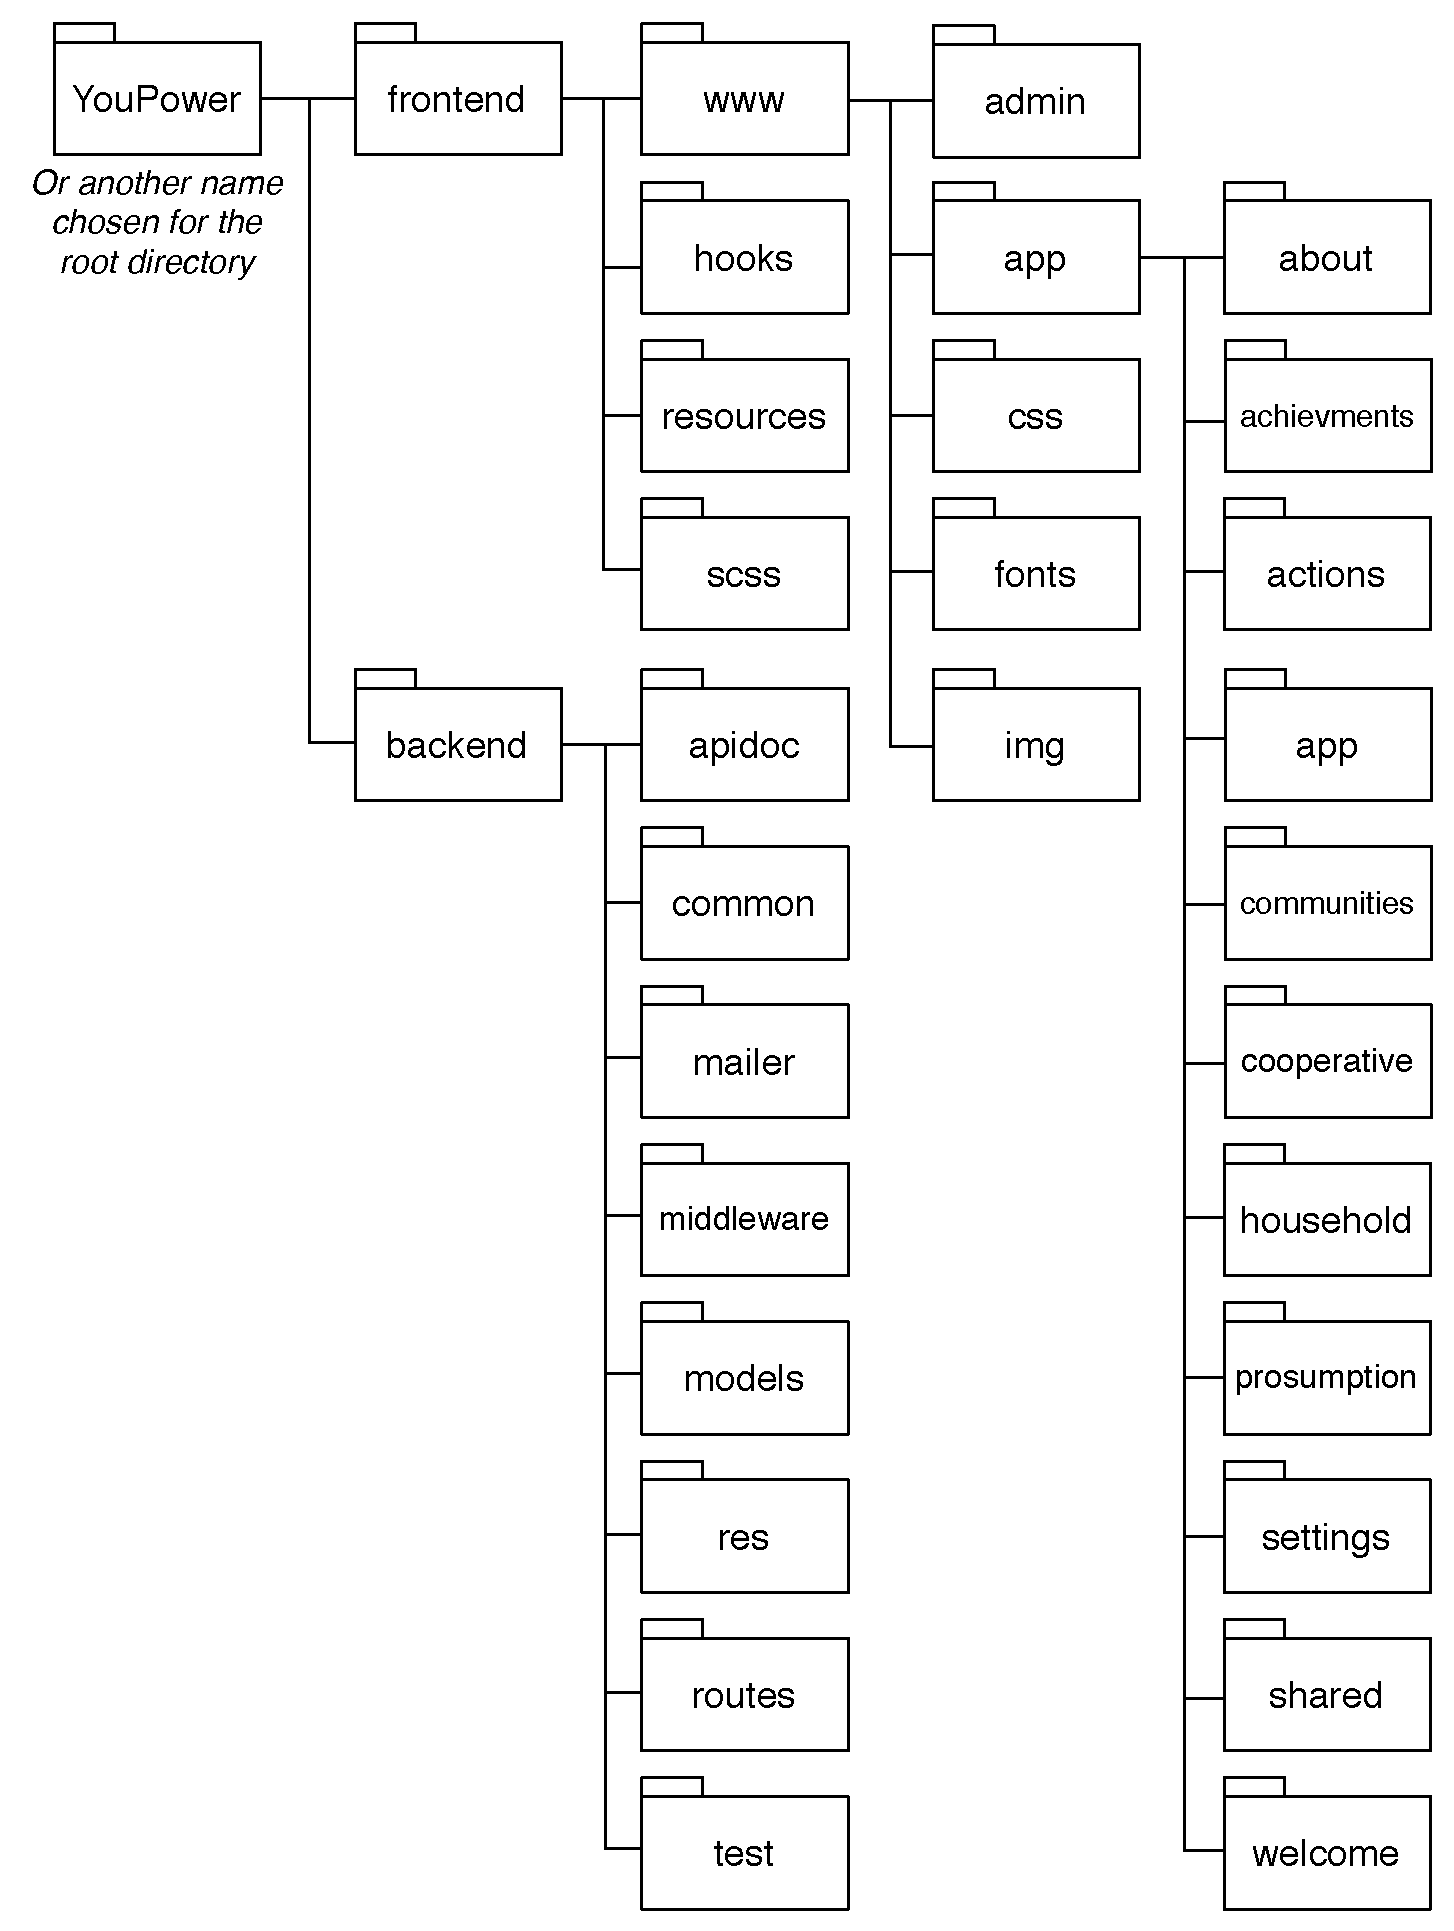
\includegraphics[width=0.9\linewidth]{img/files}
\caption{YouPower source code file structure}
\label{fig:files}
\end{figure}

\item Start MongoDB. The MongoDB installation and start process/commands are different on Linux/OSx/Windows machines. Please refer to the MongoDB manual\footnote{\url{https://docs.mongodb.com/manual/installation/\#tutorials}} for details.  

\item Start back-end server (1) with Npm start: 
\begin{lstlisting}
npm start
\end{lstlisting}
or (2) with Gulp: 
\begin{lstlisting}
gulp
\end{lstlisting}
When running the back-end with gulp, the back-end is restarted automatically if there is any change in *.js files. 

\item

\item 

\end{itemize} 


\subsection{Production Server Setup}

To setup a production server, 